\documentclass{beamer}
\usetheme{Madrid}
\usecolortheme{default}


\usepackage[T1]{fontenc}
\usepackage[utf8]{inputenc}
\usepackage{amsmath,amssymb,bm,mathtools}
\usepackage{xcolor}
\usepackage{hyperref}
\usepackage{microtype}

\graphicspath{{./figures/}}
\usepackage{booktabs}


\title[Project 1]{Project 1}
\subtitle{CS 332, Fall 2025}
\author{Ben Cole \and Koshi Harashima}
\date{8 October, 2025}

\begin{document}

\maketitle

\begin{frame}{Outline}
  \tableofcontents
\end{frame}

\AtBeginSection[]{
  \begin{frame}{Outline}
    \tableofcontents[currentsection]
  \end{frame}
}

\section{Part 1}

% Slide 2 Introductio 1: Executive Summary
\begin{frame}{Part 1}
In Part 1, 
\medskip
\begin{itemize}
  \item \textbf{Methods:} Exact Estimation and Monte Carlo Estimation.
  \item \textbf{Results:} Koshi's bid strategy($b=v-1$) did not work well, while Ben's bid strategy(almost $b = \frac{v}{2}$) worked pretty well.
  \item \textbf{Takeaways:}: Monte Carlo approximately becomes exact as the sample size increases. The better bid strategy is to bid conservatively.
\end{itemize}
\end{frame}


% Slide 3 Modeliing
\begin{frame}{Model}
\medskip
\begin{itemize}
  \item \textbf{Setting:} single-item, first-price, two bidders.
  \item \textbf{Private value:} $v\in\{10,20,\dots,100\}$. You bid $b$.
  \item \textbf{Payoff:} if win, $u=v-b$; else $u=0$.
  \item \textbf{Winning probability:}
    \[
      P_{\text{win}}(b)=P(\text{opp}<b)+\tfrac12P(\text{opp}=b).
    \]
  \item \textbf{Objective:}
    \[
      EU(v,b)=(v-b)\,P_{\text{win}}(b),\qquad b^*(v)=\arg\max_{b}EU(v,b).
    \]
  \item EU = Expected Utility,\; MC = Monte Carlo,\; opt = optimal.
\end{itemize}
\end{frame}

% ここの表記がおかしい
%要するに、vをとってきて、その後にbid strategyとして、dataから持ってくるという式をかく。
%PwinがCDFで表せるということも書かないといけない。

% Slide4: Calculation methods 
\subsection{1. winning probability and expected utility with your bids}
\begin{frame}{1-1. Calculation methods}
\medskip
\begin{itemize}
  \item \textbf{Empirical analysis:}\\
  pick $V\sim\mathrm{Unif}\{10,\dots,100\}$; sample opponent bid set $\{b_i\}_{i=1}^n$ for that $V$.
  \item \textbf{Exact estimate:}\\
  % ここの表記がおかしい
    {\centering
    \[
    \widehat{P}_{\mathrm{win}}(b)
    \;=\;\frac{\#\{b_i < b\} \;+\; \tfrac{1}{2}\#\{b_i = b\}}{n}
    \]
    \[
    \mathrm{EU}_{\mathrm{exact}}(v,b)
    \;=\; (v - b)\,\widehat{P}_{\mathrm{win}}(b)
    \]}
  \item \textbf{Monte Carlo estimator:} \\
  % ここの表記がおかしい
  draw $B_{\text{opp}}^{(t)}$ from empirical model for $t=1,\dots,T$,
    \[
      \widehat{EU}_{\text{MC}}(v,b)=\frac{1}{T}\sum_{t}\Big(\mathbf{1}\{b>B_{\text{opp}}^{(t)}\}+\tfrac12\mathbf{1}\{b=B_{\text{opp}}^{(t)}\}\Big)(v-b).
    \]
    \begin{itemize}
        \item use $T=20{,}000$ for stable MC estimates.
    \end{itemize}
\end{itemize}
\end{frame}


% Result - koshi - 
\begin{frame}{1-1. Koshi's Case}
1.Calculate your winning probability and expected utility with your bids submitted in Ex 1.2 for each of your values.
\begin{center}
\small
\begin{tabular}{@{}rrrrrrrr@{}}
\toprule
value & my bid & win prob & EU exact & EU MC & opt bid & opt EU & regret \\
\midrule
 10 &   9 & 0.091 & 0.091 & 0.088 &  5 & 0.334 & 0.243 \\
 20 &  19 & 0.252 & 0.252 & 0.250 & 11 & 1.740 & 1.487 \\
 30 &  29 & 0.418 & 0.418 & 0.417 & 11 & 3.694 & 3.276 \\
 40 &  39 & 0.577 & 0.577 & 0.580 & 21 & 6.529 & 5.952 \\
 50 &  49 & 0.716 & 0.716 & 0.718 & 21 & 9.984 & 9.268 \\
 60 &  59 & 0.805 & 0.805 & 0.806 & 31 &14.713 &13.908 \\
 70 &  69 & 0.855 & 0.855 & 0.856 & 31 &19.804 &18.949 \\
 80 &  79 & 0.905 & 0.905 & 0.904 & 41 &25.462 &24.557 \\
 90 &  89 & 0.950 & 0.950 & 0.951 & 41 &32.007 &31.057 \\
100 &  99 & 0.991 & 0.991 & 0.991 & 51 &38.675 &37.685 \\
\bottomrule
\end{tabular}
\end{center}
Koshi took a strategy in which he always bid \(b=v-1\).\\
Average Regret : \textbf{14.63}
\end{frame}


% Result - Ben -
\begin{frame}{1-1. Ben's Case}
2. Calculate your winning probability and expected utility with your bids submitted in Ex 1.2 for each of your values.
\begin{center}
\small
\begin{tabular}{@{}rrrrrrrr@{}}
\toprule
value & my bid & win prob & EU exact & EU MC & opt bid & opt EU & regret \\
\midrule
 10 &   9 & 0.091 & 0.091 & 0.088 &  5 & 0.334 & 0.243 \\
 20 &  15 & 0.216 & 1.080 & 1.075 & 11 & 1.740 & 0.660 \\
 30 &  20 & 0.291 & 2.909 & 2.865 & 11 & 3.694 & 0.785 \\
 40 &  25 & 0.375 & 5.625 & 5.569 & 21 & 6.529 & 0.904 \\
 50 &  30 & 0.455 & 9.091 & 9.089 & 21 & 9.984 & 0.893 \\
 60 &  30 & 0.455 &13.636 &13.633 & 31 &14.713 & 1.076 \\
 70 &  35 & 0.532 &18.614 &18.648 & 31 &19.804 & 1.190 \\
 80 &  40 & 0.607 &24.273 &24.406 & 41 &25.462 & 1.189 \\
 90 &  45 & 0.677 &30.477 &30.651 & 41 &32.007 & 1.530 \\
100 &  50 & 0.745 &37.273 &37.403 & 51 &38.675 & 1.403 \\
\bottomrule
\end{tabular}
\end{center}
Ben took a strategy in which he always bid almost \(b=\frac{v}{2}\).\\
Average Regret : \textbf{0.98}
\end{frame}

% Slide 7 rest of Part 1
\subsection{2. the optimal bids}
\begin{frame}{1-2. Optimal-Bids}
\begin{itemize}
    \item Calculate the optimal bids values by grid search.
    \begin{itemize}
        \item the answer is 
    \end{itemize} 
        {\small
        \begin{center}
        \begin{tabular}{@{}rrrrrrrr@{}}
        \toprule
        value & b\_opt\_exact & util\_opt\_exact & b\_opt\_mc & util\_opt\_mc \\
        \midrule
        10  &  5.1 &  0.3341 &  1.6 &  0.3507 \\
        20  & 11.1 &  1.7395 & 11.1 &  1.8067 \\
        30  & 11.1 &  3.6941 & 11.1 &  3.8367 \\
        40  & 21.1 &  6.5291 & 21.6 &  6.6608 \\
        50  & 21.1 &  9.9836 & 21.6 & 10.2808 \\
        60  & 31.1 & 14.7127 & 31.3 & 14.9455 \\
        70  & 31.1 & 19.8036 & 31.3 & 20.1530 \\
        80  & 41.1 & 25.4618 & 41.0 & 25.8814 \\
        90  & 41.1 & 32.0073 & 41.0 & 32.5176 \\
        100 & 51.1 & 38.6755 & 41.0 & 39.1539 \\
        \bottomrule
        \end{tabular}
        \end{center}}
\end{itemize}
\end{frame}

\begin{frame}{1-2. Example}
    \begin{figure}
        \centering
        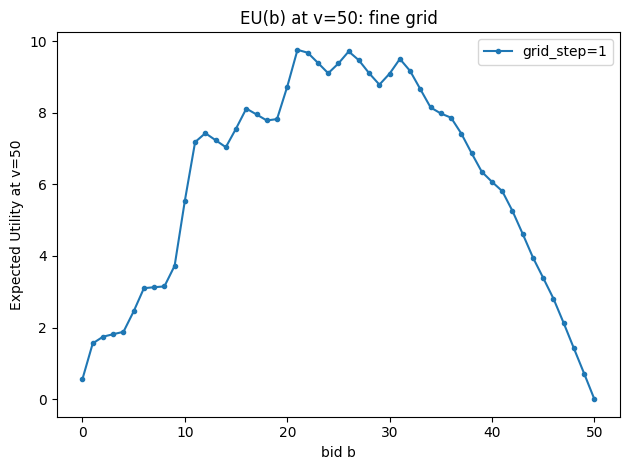
\includegraphics[width=0.6\linewidth]{332Project1//figures/EU_plot_revised.png}
        \caption{Change of Expected Utility when my value is 50}
        \label{fig:placeholder}
    \end{figure}
    According to Figure, we concluded that the optimal bid is around 20 or 30 when the value is 50 
\end{frame}

\subsection{3. Better bid strategy}
\begin{frame}{1-3.Better bid Strategy}
\begin{itemize}
    \item Compare the utility you obtained to the optimal utility you could have obtained.  Can you conclude anything about a good strategy in this auction?
    \begin{itemize}
        \item from Koshi's case: we observe that it is not recommended to bid too close to your valuation.
        \item From Ben's case: he bids conservatively, yet his bids are close to the optimal bids and show very good expected-utility performance.
        \end{itemize}
\end{itemize}
\vspace{0.5em}
\begin{columns}[t]
  \begin{column}{0.48\textwidth}
    \centering
    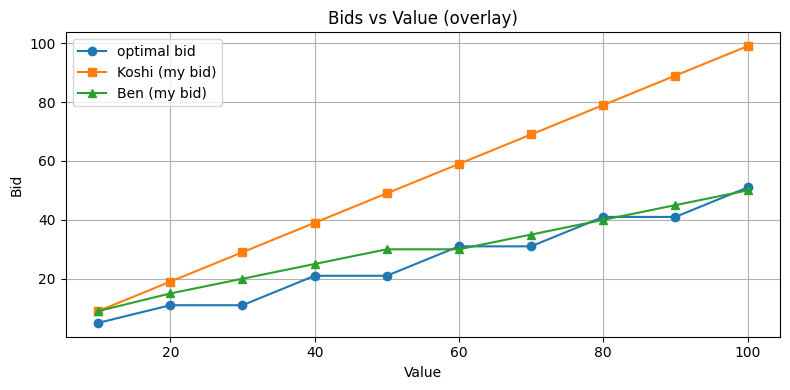
\includegraphics[width=\linewidth]{332Project1/figures/bid_revised.png}
    \vspace{0.4em}
    {\footnotesize (a) Bid vs.\ value}
  \end{column}
  \begin{column}{0.48\textwidth}
    \centering
    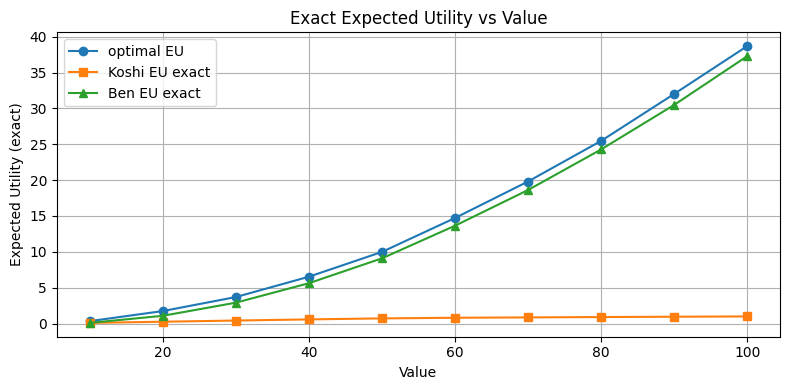
\includegraphics[width=\linewidth]{332Project1/figures/EU_revised.png}
    \vspace{0.4em}
    {\footnotesize (b) Expected utility vs.\ value}
  \end{column}
\end{columns}
\end{frame}

\begin{frame}{1-3. Appendix: Regret}
    \begin{figure}
        \centering
        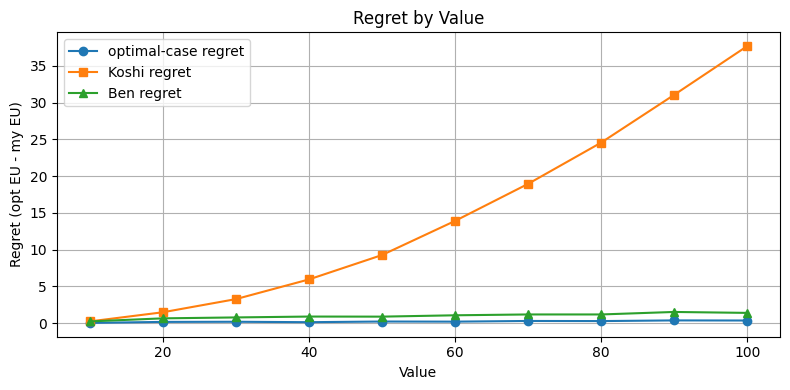
\includegraphics[width=1\linewidth]{332Project1/figures/regret.png}
    \vspace{0.4em}
    {\footnotesize (c) Regret}
    \end{figure}
\end{frame}

\section{Part 2}

\begin{frame}{Part 2}
    In Part 2, we consider two things; 
    \medskip
    \begin{itemize}
        \item 1. Optimal data-driven bid strategy (stated in CANVAS)
        \item 2. The theoretically optimal bid in a two-player First-price auction
    \end{itemize}
\end{frame}

\subsection{1. optimal data-driven bid strategy}

\begin{frame}{2-1. Summary}
\small
\textbf{Method:}
\begin{itemize}
    \item We then analyze how the empirical estimates converge to the true distribution as the sample size increases.
\end{itemize}
\textbf{Results:}
\begin{itemize}
    \item The optimal bidding algorithm is obtained by choosing the bid function, and F(b) can be estimated through data.
    \[
    b^*(v) = \arg\max_{b}(v-b)F(b).
    \]
    \item As the number of bid samples increases, the variance of the estimated expected utility decreases,
    leading to more accurate estimation of the opponent’s bidding strategy and convergence of $\hat b^*(v)$ to $b^*(v)$.
\end{itemize}
\textbf{Takeaway.}\\
\begin{itemize}
    \item More bid samples lead to a smoother, more accurate $\hat F$\\
    \item $\Rightarrow$ obtain bid strategy that converge to the true optimal policy.
    \item This analysis can be applied to arbitral type of distribution.
\end{itemize}
\end{frame}

%Summary
\begin{frame}{2-1. Setup}
\small
\textbf{Setting.}
\begin{itemize}
  \item Same auction environment as in Part 1.
  \item Algorithm chooses a bid function $b(v)$ that maximizes expected utility.
\end{itemize}

\vspace{1em}

\textbf{Formulation of bid algorithm problem.}\\
\begin{itemize}
    \item Creating the algorithm which chooses a bid function $b(v)$ to maximize expected utility(in other words, choose the empirical optimal strategy):
    \begin{align*}
    b^*(v) = \arg\max_b (v-b)\,\Pr(B_{\text{opp}}\le b)
    \end{align*}
    \item In our setting, value is parameterized discretely, so our goal is to find the optimal bid $b^*$ for each value $v (=10, 20, \dots, 100)$.
    \item To avoid notational confusion, this presentation does not include analysis of cases in which items are randomly assigned between the two players when tie.\\
    \item Note that the discussion still holds even when tie cases are included 
\end{itemize}
\end{frame}

\begin{frame}{2-1. Method}
\small
\textbf{Win Probability. $\Pr(B_{\text{opp}}\le b)$}\\
Your win probability is the probability that the opponent's bid $B_{opp}$
is below your bid $b$:
\[
\Pr(B_{\text{opp}}\le b).
\]
This probability comes from two components:
\begin{itemize}
    \item the distribution of the opponent’s value $V_{\text{opp}}$, and
    \item the opponent’s bidding function $b_{\text{opp}}(V_{\text{opp}})$
\end{itemize}
\end{frame}

\begin{frame}{2-1. Method}
\small
\textbf{What we estimate is win probability}
\begin{itemize}
  \item For each $v'_i$(drawn from uniform distribution), we observe $n$ bids $B_{i,1},\dots,B_{i,n}$ from the dataset (\texttt{bid\_data.csv}, and in ur experiment, n=22).
  \item Per value CDF:
  \[
  \hat G_{v'_i}(b)=\frac{1}{n}\sum_{j=1}^n \mathbf{1}\{B_{i,j}\le b\}.
  \]
  \item For each valuation level $v'_i$, we observe $n$ bids
  \[
    \{B_{i,1},\dots,B_{i,n}\}\ \text{i.i.d.}\sim G_{v'_i},
  \]
    where $G_{v'_i}(b)=\Pr(B_{\text{opp}}\le b\mid V_{\text{opp}}=v'_i)$
    is the conditional bid distribution.
  \item Aggregate CDF:
  \[
    \hat F(b)=\frac{1}{10}\sum_{i=1}^{10}\hat G_{v'_i}(b).
  \]
  \item Therefore, our bid algorithm problem can be formulated as follows.
  \[
    \hat b^*(v)\in\arg\max_{b}(v-b)\,\hat F(b).
  \]
\end{itemize}
\end{frame}

\begin{frame}{2-1. Statistical Method}
\small
\textbf{Estimator (per value)}
\begin{align*}
  \hat{G}_{v'_i}(b)
    &= \frac{1}{n}\sum_{j=1}^{n}\mathbf{1}\{B_{i,j}\le b\}, \\[4pt]
  \mathbb{E}[\hat{G}_{v'_i}(b)]
    &= G_{v'_i}(b), \\[4pt]
  \mathrm{Var}[\hat{G}_{v'_i}(b)]
    &= \frac{G_{v'_i}(b)\bigl(1-G_{v'_i}(b)\bigr)}{n}.
\end{align*}

\textbf{Aggregated win CDF}
\begin{align*}
  F(b) &= \frac{1}{10}\sum_{i=1}^{10} G_{v'_i}(b),\quad
  \hat{F}(b) = \frac{1}{10}\sum_{i=1}^{10} \hat{G}_{v'_i}(b).
\end{align*}

Hence,
\[
  \mathbb{E}[\hat{F}(b)] = F(b), 
  \quad
  \mathrm{Var}[\hat{F}(b)] = O\!\left(\frac{1}{n}\right).
\]
\end{frame}


\begin{frame}{2-1. Results (in theory)}
\textbf{Implication.}\\
As $n$ increases, the variance of the estimator decreases
while its expected value remains unchanged.
Therefore, our estimate of the opponent’s bidding strategy
becomes more precise, and the optimal bid converges to the true one:
\[
\hat b^*(v)=\arg\max_{b}(v-b)\,\hat F(b)
\ \longrightarrow\
b^*(v)=\arg\max_{b}(v-b)\,F(b).
\]
\end{frame}

\begin{frame}{2-1. Results (in empirical)}
\begin{itemize}
    \item Here are the examples of Per value CDF.\\
    \item These figures shows culumulatice distribution functions given V. Vertical axis shows the amount of bid and horizontal axis shows that its culumulative density.
\end{itemize}
\begin{columns}[T,onlytextwidth]
  \column{0.33\textwidth}
  \begin{figure}
    \centering
    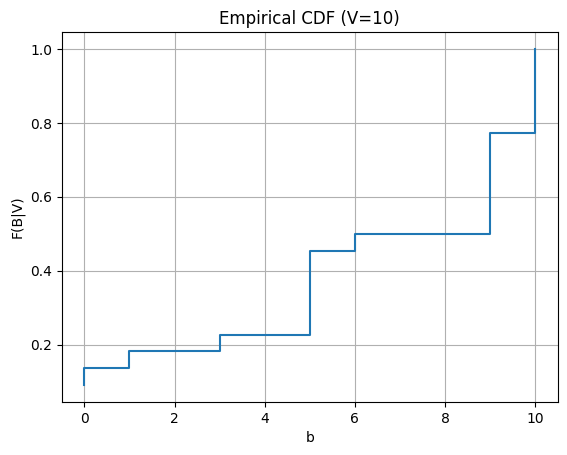
\includegraphics[width=\linewidth]{332Project1/figures/v=10.png}
    \caption{V=10}\label{fig:v10}
  \end{figure}

  \column{0.33\textwidth}
  \begin{figure}
    \centering
    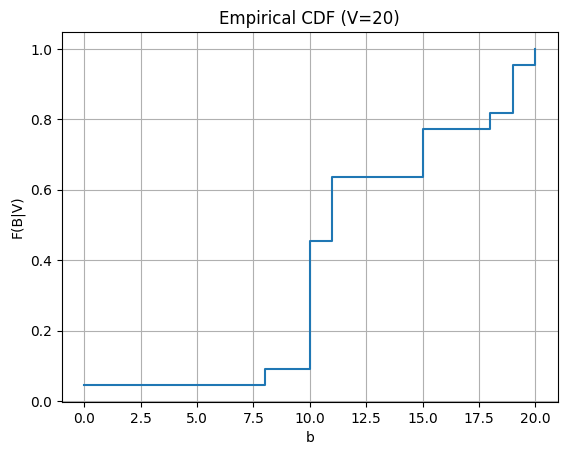
\includegraphics[width=\linewidth]{332Project1/figures/v=20.png}
    \caption{V=20}\label{fig:v20}
  \end{figure}

  \column{0.33\textwidth}
  \begin{figure}
    \centering
    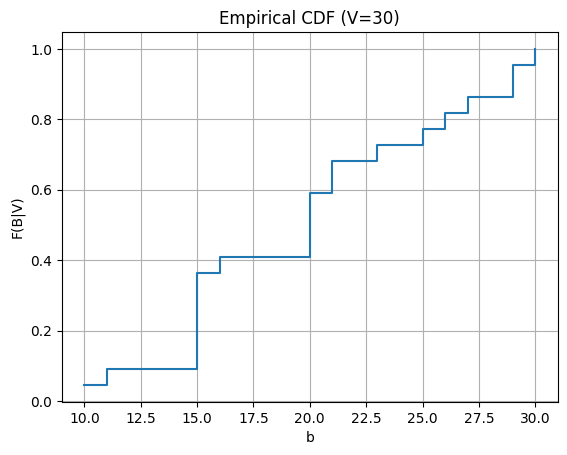
\includegraphics[width=\linewidth]{332Project1/figures/v=30.png}
    \caption{V=30}\label{fig:v30}
  \end{figure}
\end{columns}
\end{frame}

\begin{frame}{2-1. Results (in empirical)}
\begin{itemize}
    \item Here are the examples of Aggregated CDF.
    \item We assume a uniform distribution, so treat all bids in samples equally.
    \item Therefore, the aggregated CDF is equivalent to constructing a cumulative distribution that gives equal weight to all observed samples (in our experiment, 22×10 samples in total)
    \item Vertical axis shows the amount of bid and horizontal axis shows that its culumulative density.
\end{itemize}
\begin{figure}
    \centering
    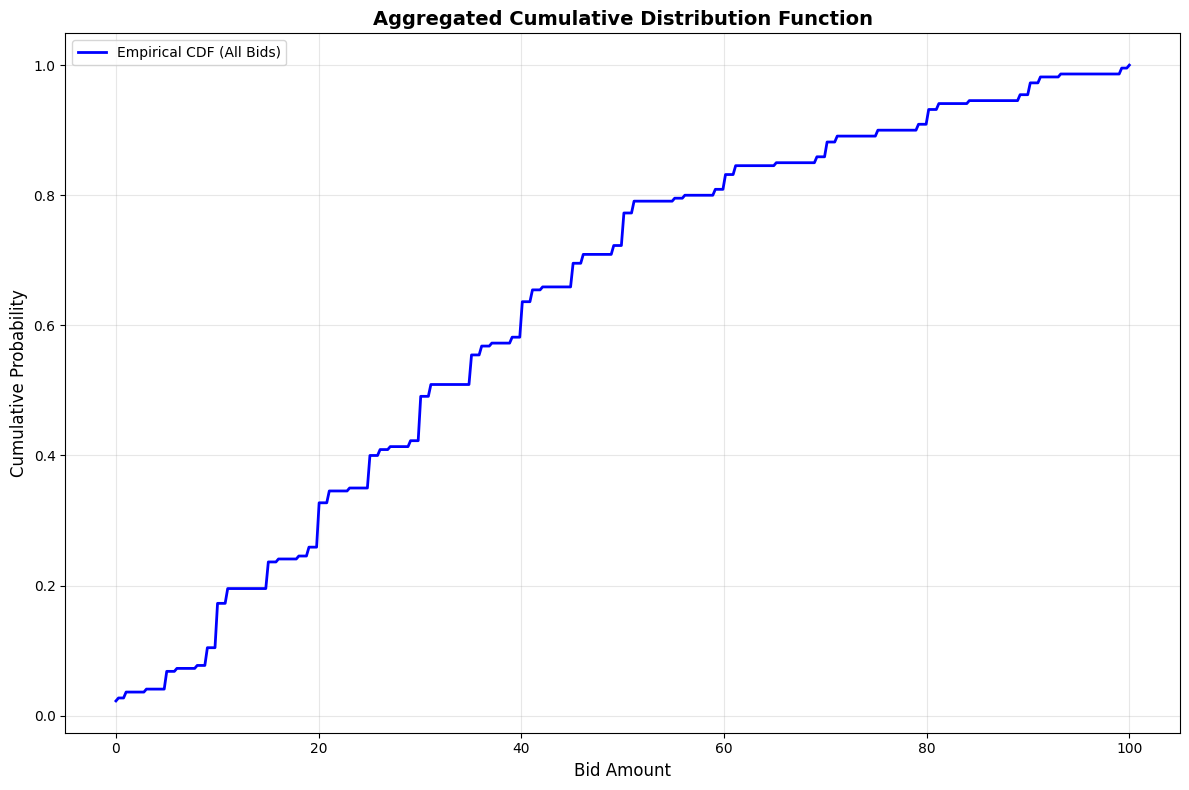
\includegraphics[width=0.4\linewidth]{332Project1//figures/AggregatedCDF.png}
    \caption{Aggregated CDF}
    \label{fig:placeholder}
\end{figure}
\end{frame}

\begin{frame}{2-1. Appendix: Distribution(V=10,20,30)}
    \begin{figure}
        \centering
        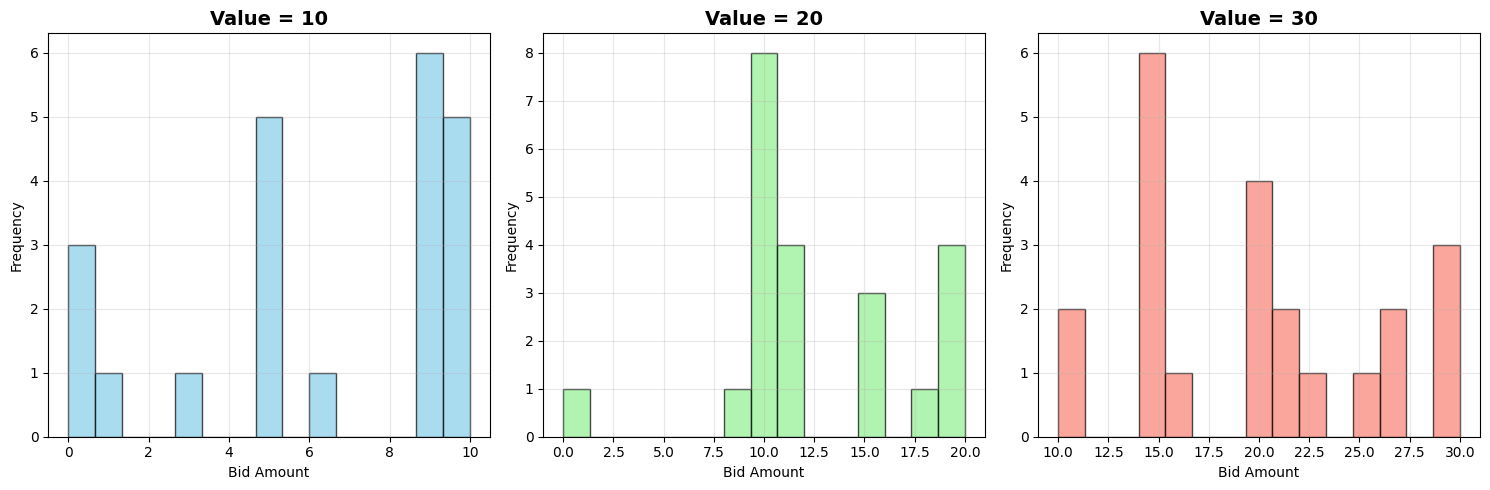
\includegraphics[width=0.7\linewidth]{332Project1/figures/barplot.png}
        \caption{Discrete Distribution}
        \label{fig:placeholder}
    \end{figure}
    \begin{figure}
        \centering
        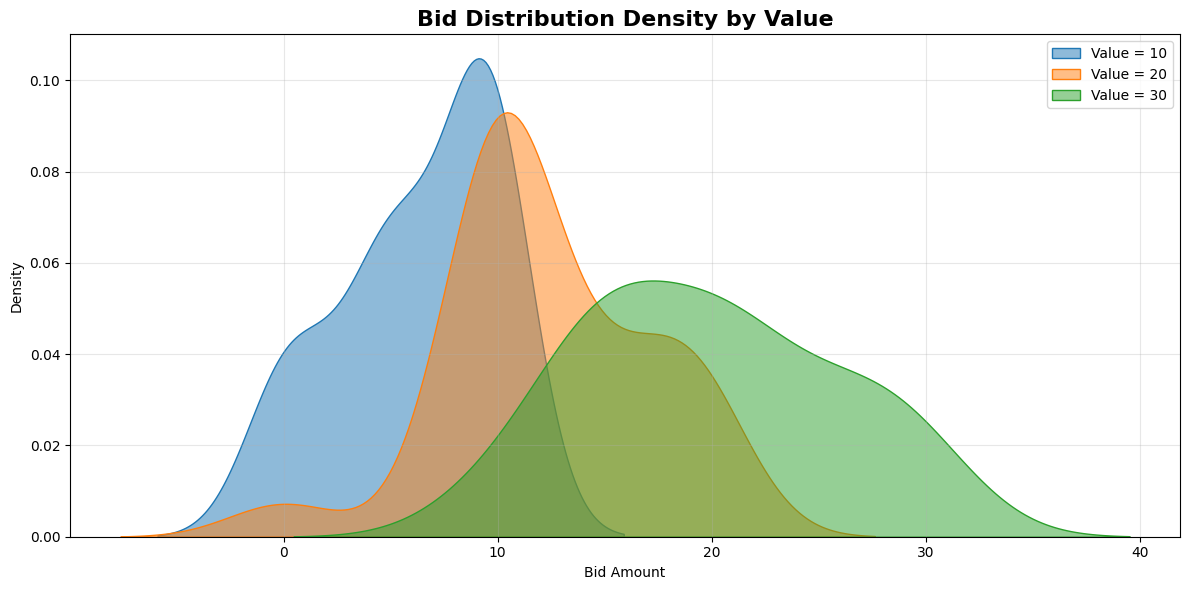
\includegraphics[width=0.5\linewidth]{332Project1/figures/Distribution.png}
        \caption{Continuous Distribution}
        \label{fig:placeholder}
    \end{figure}
\end{frame}

\subsection{2. The theoretically optimal bid in a two-player First-price auction}

\begin{frame}{2-2. Observation of the optimal bid}
\small
\begin{itemize}
  \item \textbf{First-price Auction:} : It seems like the optimal bid is linear in value, but its coefficient is half not 1(truthful).\\
  \item From this, we wondered whether this bidding strategy would be optimal in this particular setting.
\end{itemize}
\begin{figure}
    \centering
    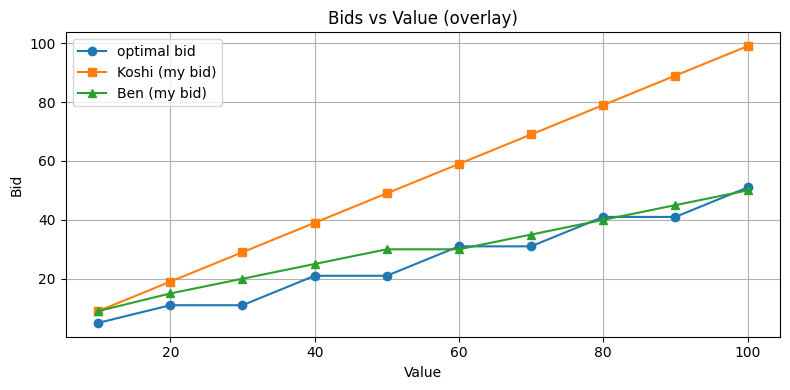
\includegraphics[width=0.7\linewidth]{332Project1/figures/bid_revised.png}
    \caption{Comparing bid strategy}
    \label{fig:placeholder}
\end{figure}
\end{frame}

\begin{frame}{2-2. Bid Strategy in First-Price Auction}
\small
\textbf{Setup:} \\
\begin{itemize}
    \item First-price Auction
    \item Two bidders, values drawn from $U[0,1]$ i.i.d.
    \item The valuation takes continuous values for simplicity, instead of discrete.
\end{itemize}

\textbf{Method:}
\begin{itemize}
    \item I made certain assumptions and,
    \item based on the best response functions and first-order conditions, derived the Nash equilibrium through simple algebraic manipulation.
\end{itemize} 
\textbf{Results:}
\begin{itemize}
    \item Assumption: opponent's bid strategy is deterministic and linear in his value.
    \item Best bid strategy is $b(v) = \frac{v}{2}$.
    \item From our empirical research so far, this strategy is robust.
\end{itemize}
\end{frame}

\begin{frame}{2-2. Calculation process}
\begin{itemize}
    \item I assume that opponent's bid strategy is deterministic and linear in his value($b(x)=\alpha x$).
    \item Optimal bid problem is formulated by following formula;
    \begin{equation*}
        b^{*}=\arg\max_{b}\,(v-b)\,\Pr(b \leq b_{opp})
    \end{equation*}
    \item Considering Best respond to a opponent, 
    \begin{equation*}
        \Pr(\text{win at bid }b)=\Pr(\alpha X<b)=\tfrac{b}{\alpha}
    \end{equation*}
    \item so, 
    \begin{equation*}
        b^{*}=\arg\max_{b}(v-b)\tfrac{b}{\alpha}\quad (= U).
    \end{equation*}
    \item First-Order Condition in b:\\
    \begin{equation*}
    \partial U/\partial b=\tfrac{1}{\alpha}(v-2b)=0 \;\ \Rightarrow\; b^*(v)=\tfrac12 v.
    \end{equation*}
    \item By symmetry, 
    \begin{equation*}
        b(v)=\alpha v=b^*(v) \ \Rightarrow\; \alpha=\frac{1}{2}.
    \end{equation*}
\end{itemize}
\end{frame}

\section{Usage of AI}
\begin{frame}{Usage of AI}
    AI was used for coding; final review and responsibility by the authors.
\end{frame}

\end{document}
